\documentclass[final]{beamer} % beamer 3.10: do NOT use option hyperref={pdfpagelabels=false} !
  %\documentclass[final,hyperref={pdfpagelabels=false}]{beamer} % beamer 3.07: get rid of beamer warnings
  \mode<presentation> { \usetheme{UFPoster} }
  \usepackage[english]{babel}
  \usepackage[latin1]{inputenc}
  \usepackage{amsmath,amsthm, amssymb, latexsym}
  \usefonttheme[onlymath]{serif}
  \boldmath
  \usepackage[orientation=portrait,size=a0,scale=1.1,debug]{beamerposter}                       % e.g. for DIN-A0 poster
  \title[Epi. on Emp. Nets]{Epidemics on Dynamic,\\ Empirical Networks}
  \author[Pearson \& Hladish]{Carl A.~B.~Pearson \&\ Thomas J.~Hladish}
  \institute[EPI-UF]{Emerging Pathogens Institute, University of Florida}
  \date{\today}
  \newcommand{\spaceProp}{0.02}
  \newcommand{\spacer}{\begin{column}{\spaceProp\paperwidth}\end{column}}
  
  \newenvironment{oneCol}{\begin{column}[t]{0.225\paperwidth}}{\end{column}}
  \newenvironment{threeCol}{\begin{column}[t]{0.715\paperwidth}}{\end{column}}
  \setbeamertemplate{caption}[numbered]
\usepackage{Sweave}
\begin{document}
\input{poster-concordance}
  \begin{frame}{}
    \begin{columns}[t]
    \spacer{}
    \begin{oneCol}
    \begin{block}{Introduction}
Contact networks are \textbf{intrinsically temporal}, but often analyzed as \textbf{time-aggregated} to simplify analysis and simulation.  Simulation on empirical networks, however, can incorporate temporal changes with minimal additional complexity.

We consider such simulation on $\mathbf{\approx 2\times 10^6}$\textbf{ nodes}, interacting via $\mathbf{\approx 2\times 10^6}$\textbf{ edges}, \textbf{over 5-years} of geo-temporal co-location data, derived from municipal WiFi access at businesses in Montreal\cite{hoen2013montreal}.  We start with a \textbf{review of network measures for different aggregation windows} on that data, and \textbf{conclude comparing simulated infections on these dynamic networks}.
%     \begin{block}{\large Fontsizes}
%       \centering
%       {\tiny tiny}\par
%       {\scriptsize scriptsize}\par
%       {\footnotesize footnotesize}\par
%       {\normalsize normalsize}\par
%       {\large large}\par
%       {\Large Large}\par
%       {\LARGE LARGE}\par
%       {\veryHuge veryHuge}\par
%       {\VeryHuge VeryHuge}\par
    \end{block}
    \begin{block}{Materials}
Data preparation with R and Scala.  Network analysis and epidemic simulation with EpiFire\cite{hladish2012epifire} (new features to be formally documented in future publication, development code now available).  Visualization and poster with R and \LaTeX; non-EpiFire source @ \href{https://github.com/pearsonca/epidemics4-talk}{github.com/pearsonca/epidemics4-talk}.
    \end{block}
    \begin{block}{Methods}
The raw data have three issues: some logouts before logins, missing logout times, and overlapping logins for a single user at a location.  The first issue was resolved by swapping the times; this affected $\approx 10$ rows, and the swapped durations were consistent with other durations for those users.  For the missing logout times, we set them to their login times; this still allows those visits to intersect with other users.  Finally, we union each user's login periods to address concurrent use from multiple devices.

The network measures for reference are the maximum component size and maximum degree, computed using the edge configuration in each time period.  An edge exists between individuals if their access at a location overlaps in time.

The epidemic is an \textbf{S$\rightarrow$E$\rightarrow$I$\rightarrow$R$\rightarrow$S} model, simulated given five parameters:\begin{itemize}
\item contact rate, $\beta = 2.0$ contacts/day,
\item latent period, $\mu = 1.2$ days,
\item infectious period, $\gamma = 4.1$ days
\item resistant period, $\omega = 365$ days
\item and the infectious seeding rate, $\sigma_I = 0.1$ per day
\end{itemize}

We selected $\mu$, $\gamma$, and $\omega$ from literature estimates for influenza.  The resistant (immune) duration is the same for all individuals; other state durations are exponentially distributed.  As each individual is infected, contact and state transition times are generated.  As time passes, edges are added and removed when binning boundaries are reached.  At contact times, a contact is chosen from the edges that exist at that moment. 
    \end{block}
    \begin{block}{Conclusion}
The aggregation window for social network observations can determine the type of infectious dynamics that are possible to simulate for given parameters.
    \end{block}
    \begin{block}{References}
      \nocite{*} % Insert publications even if they are not cited in the poster
      \small{\bibliographystyle{unsrt}
      \bibliography{biblio}\vspace{0.75in}}
    \end{block}
    \end{oneCol}
    \spacer{}
    \begin{threeCol}
    \begin{block}{Source Data Overview}
    \begin{columns}
    \begin{oneCol}
      \begin{figure}
        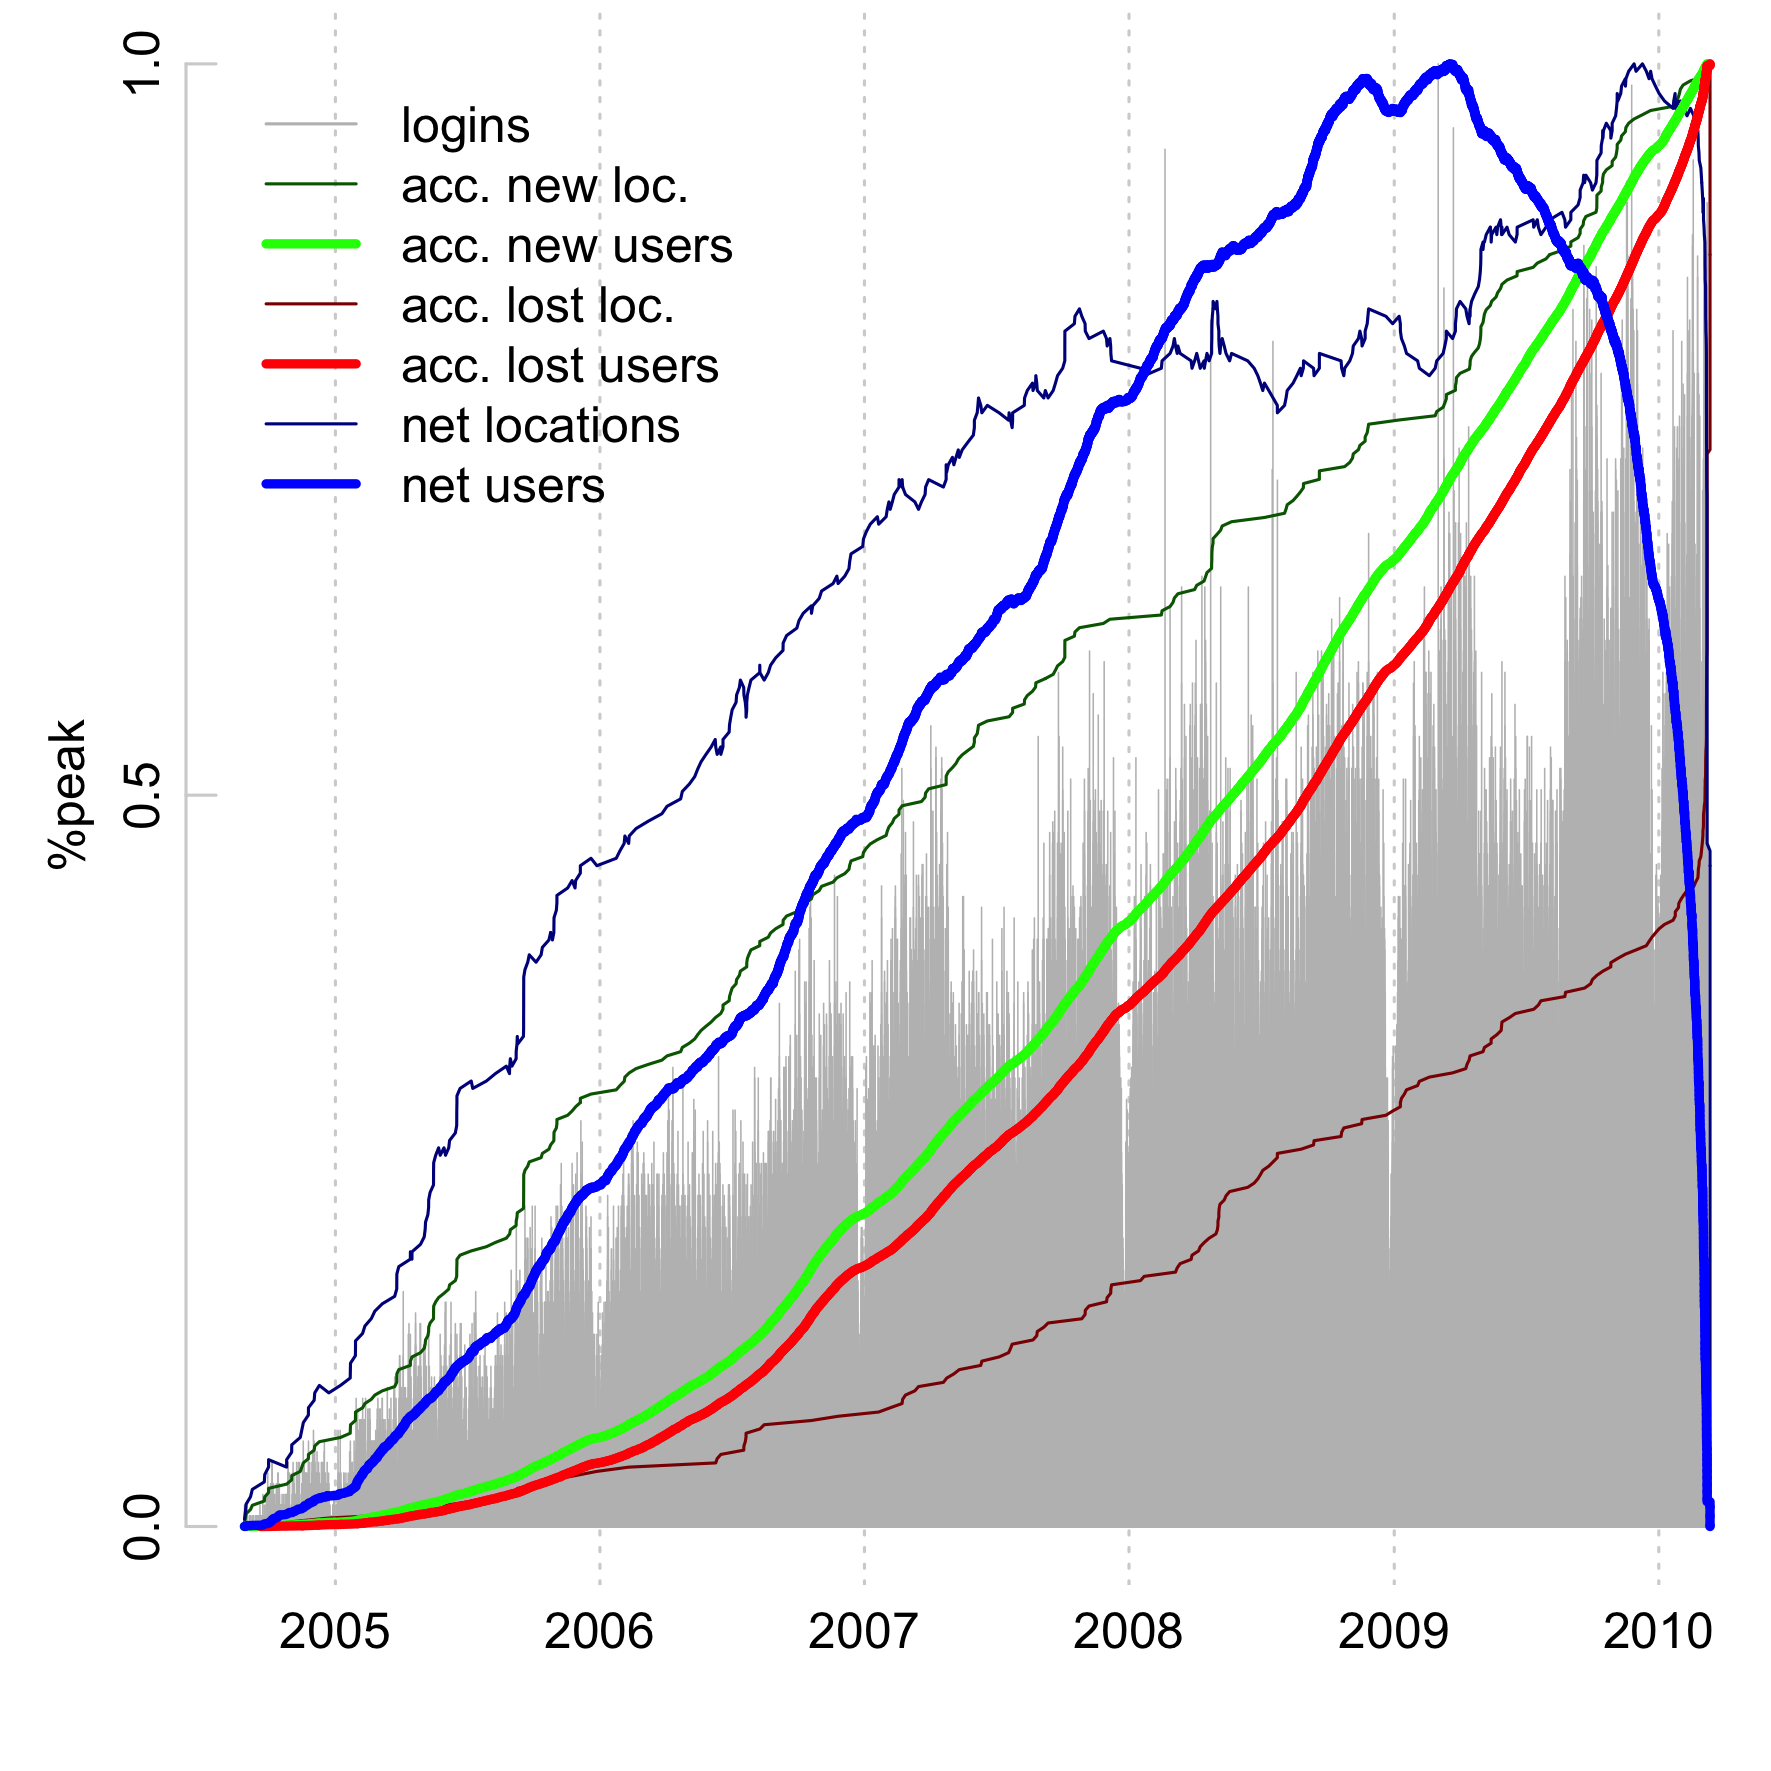
\includegraphics[width=1.0\linewidth]{dataReview.png}
      \end{figure}   
    \end{oneCol}
    %\spacer{}
    \begin{oneCol}
      \begin{figure}
        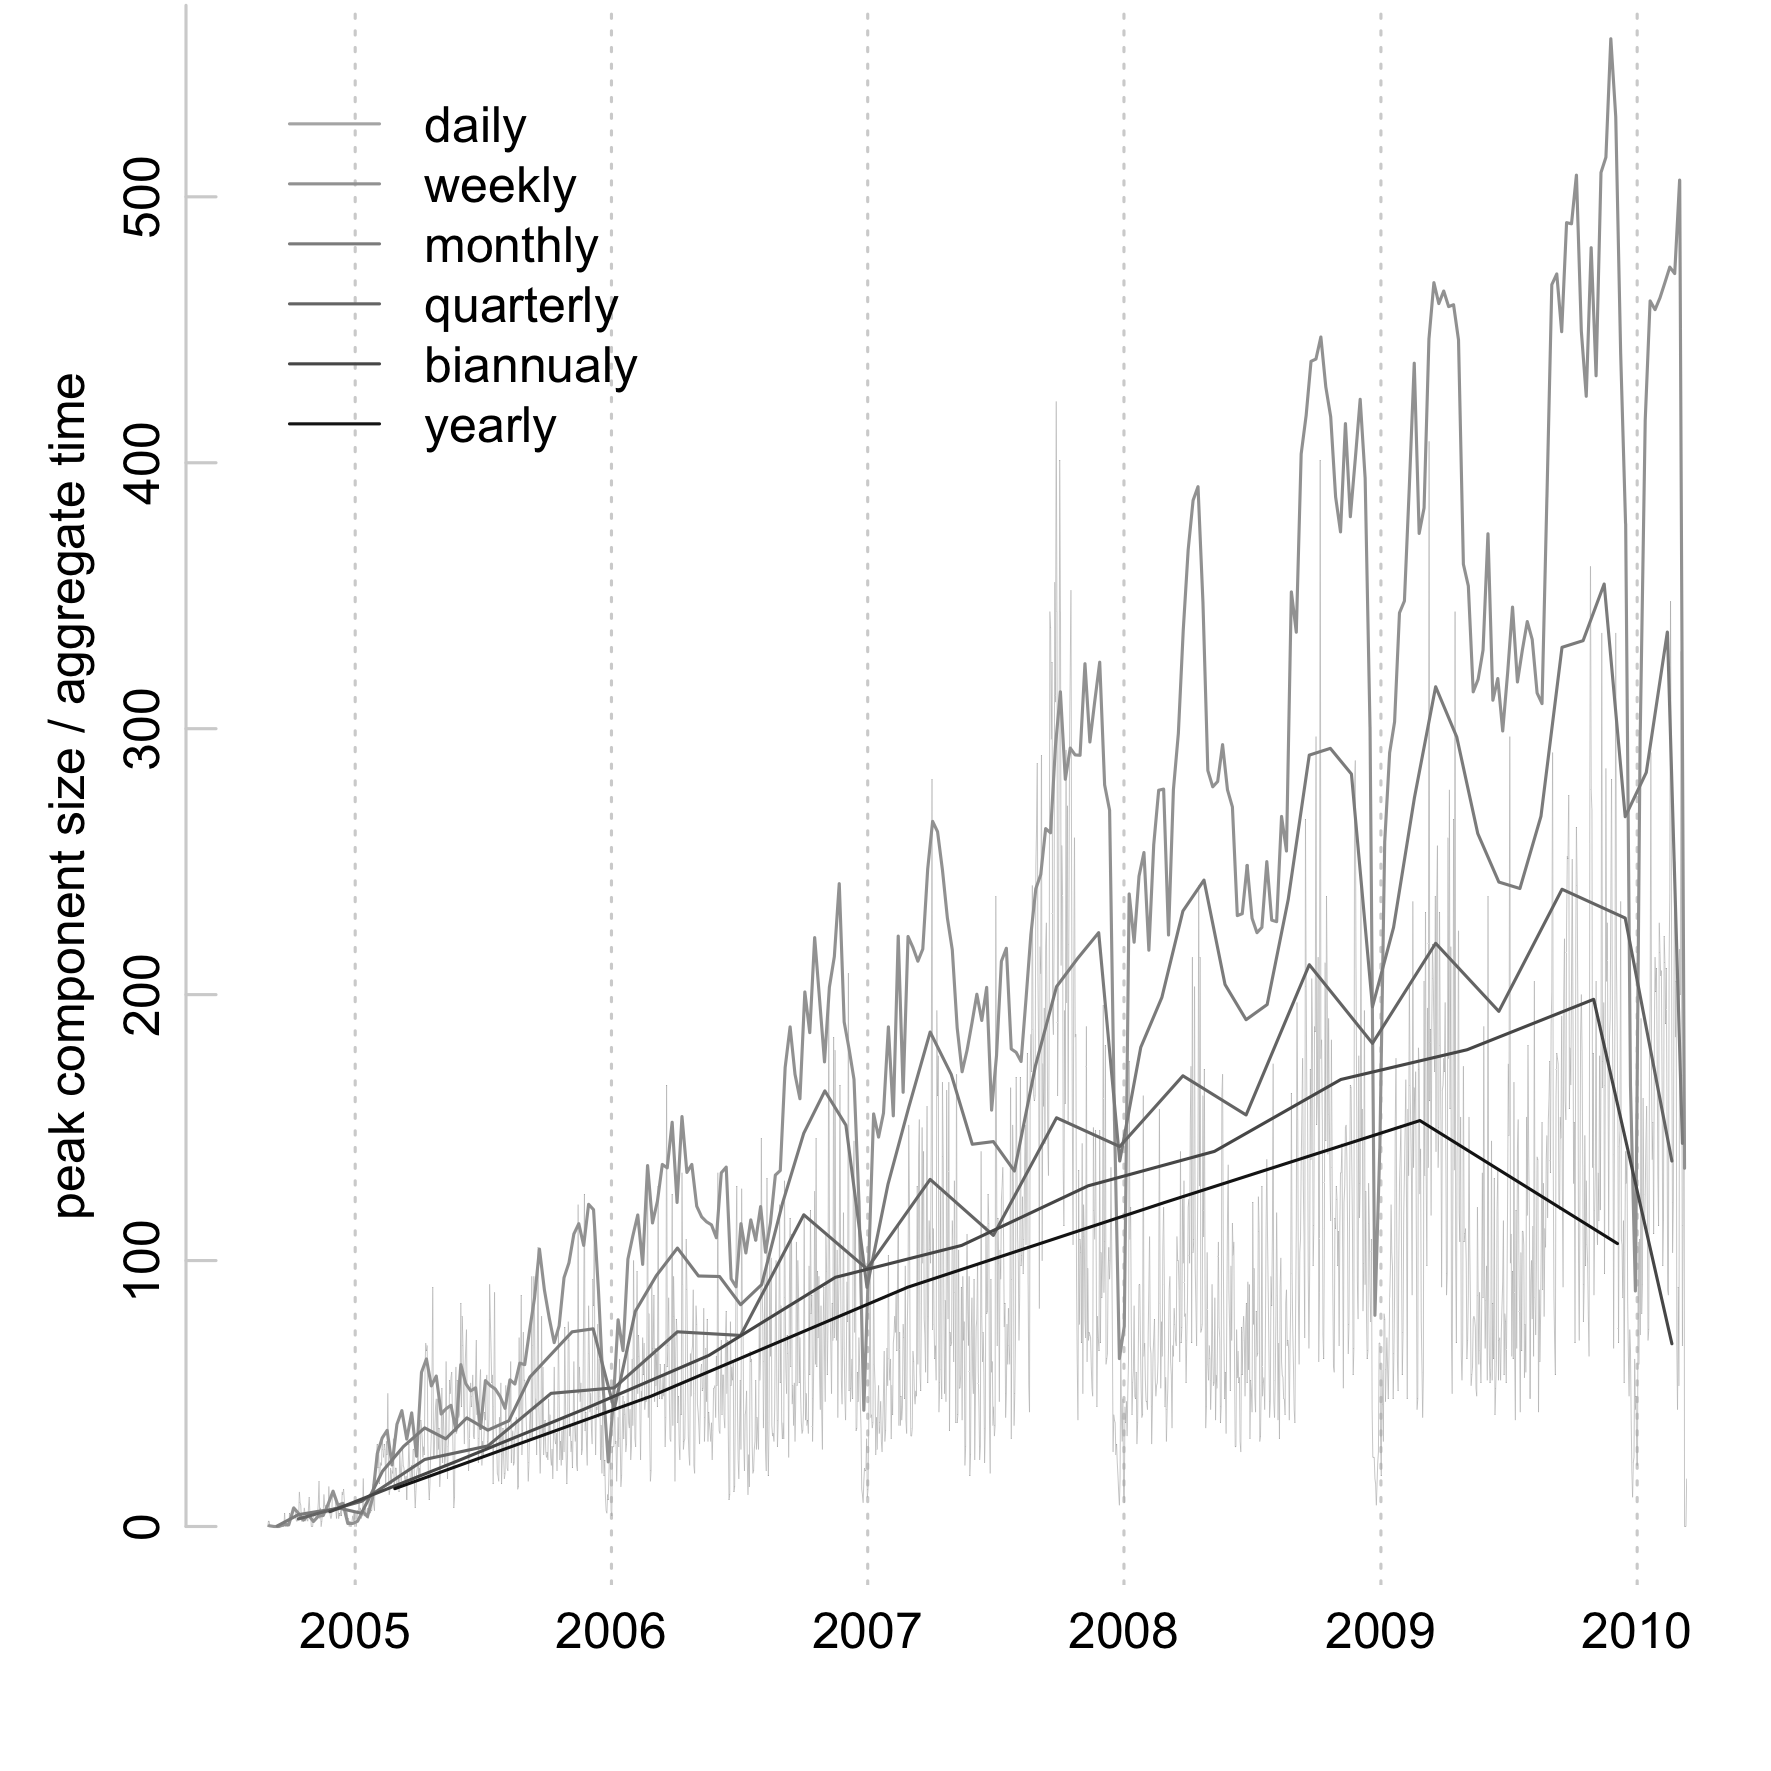
\includegraphics[width=1.0\linewidth]{maxComp.png}
      \end{figure}   
    \end{oneCol}
    %\spacer{}
    \begin{oneCol}
      \begin{figure}
        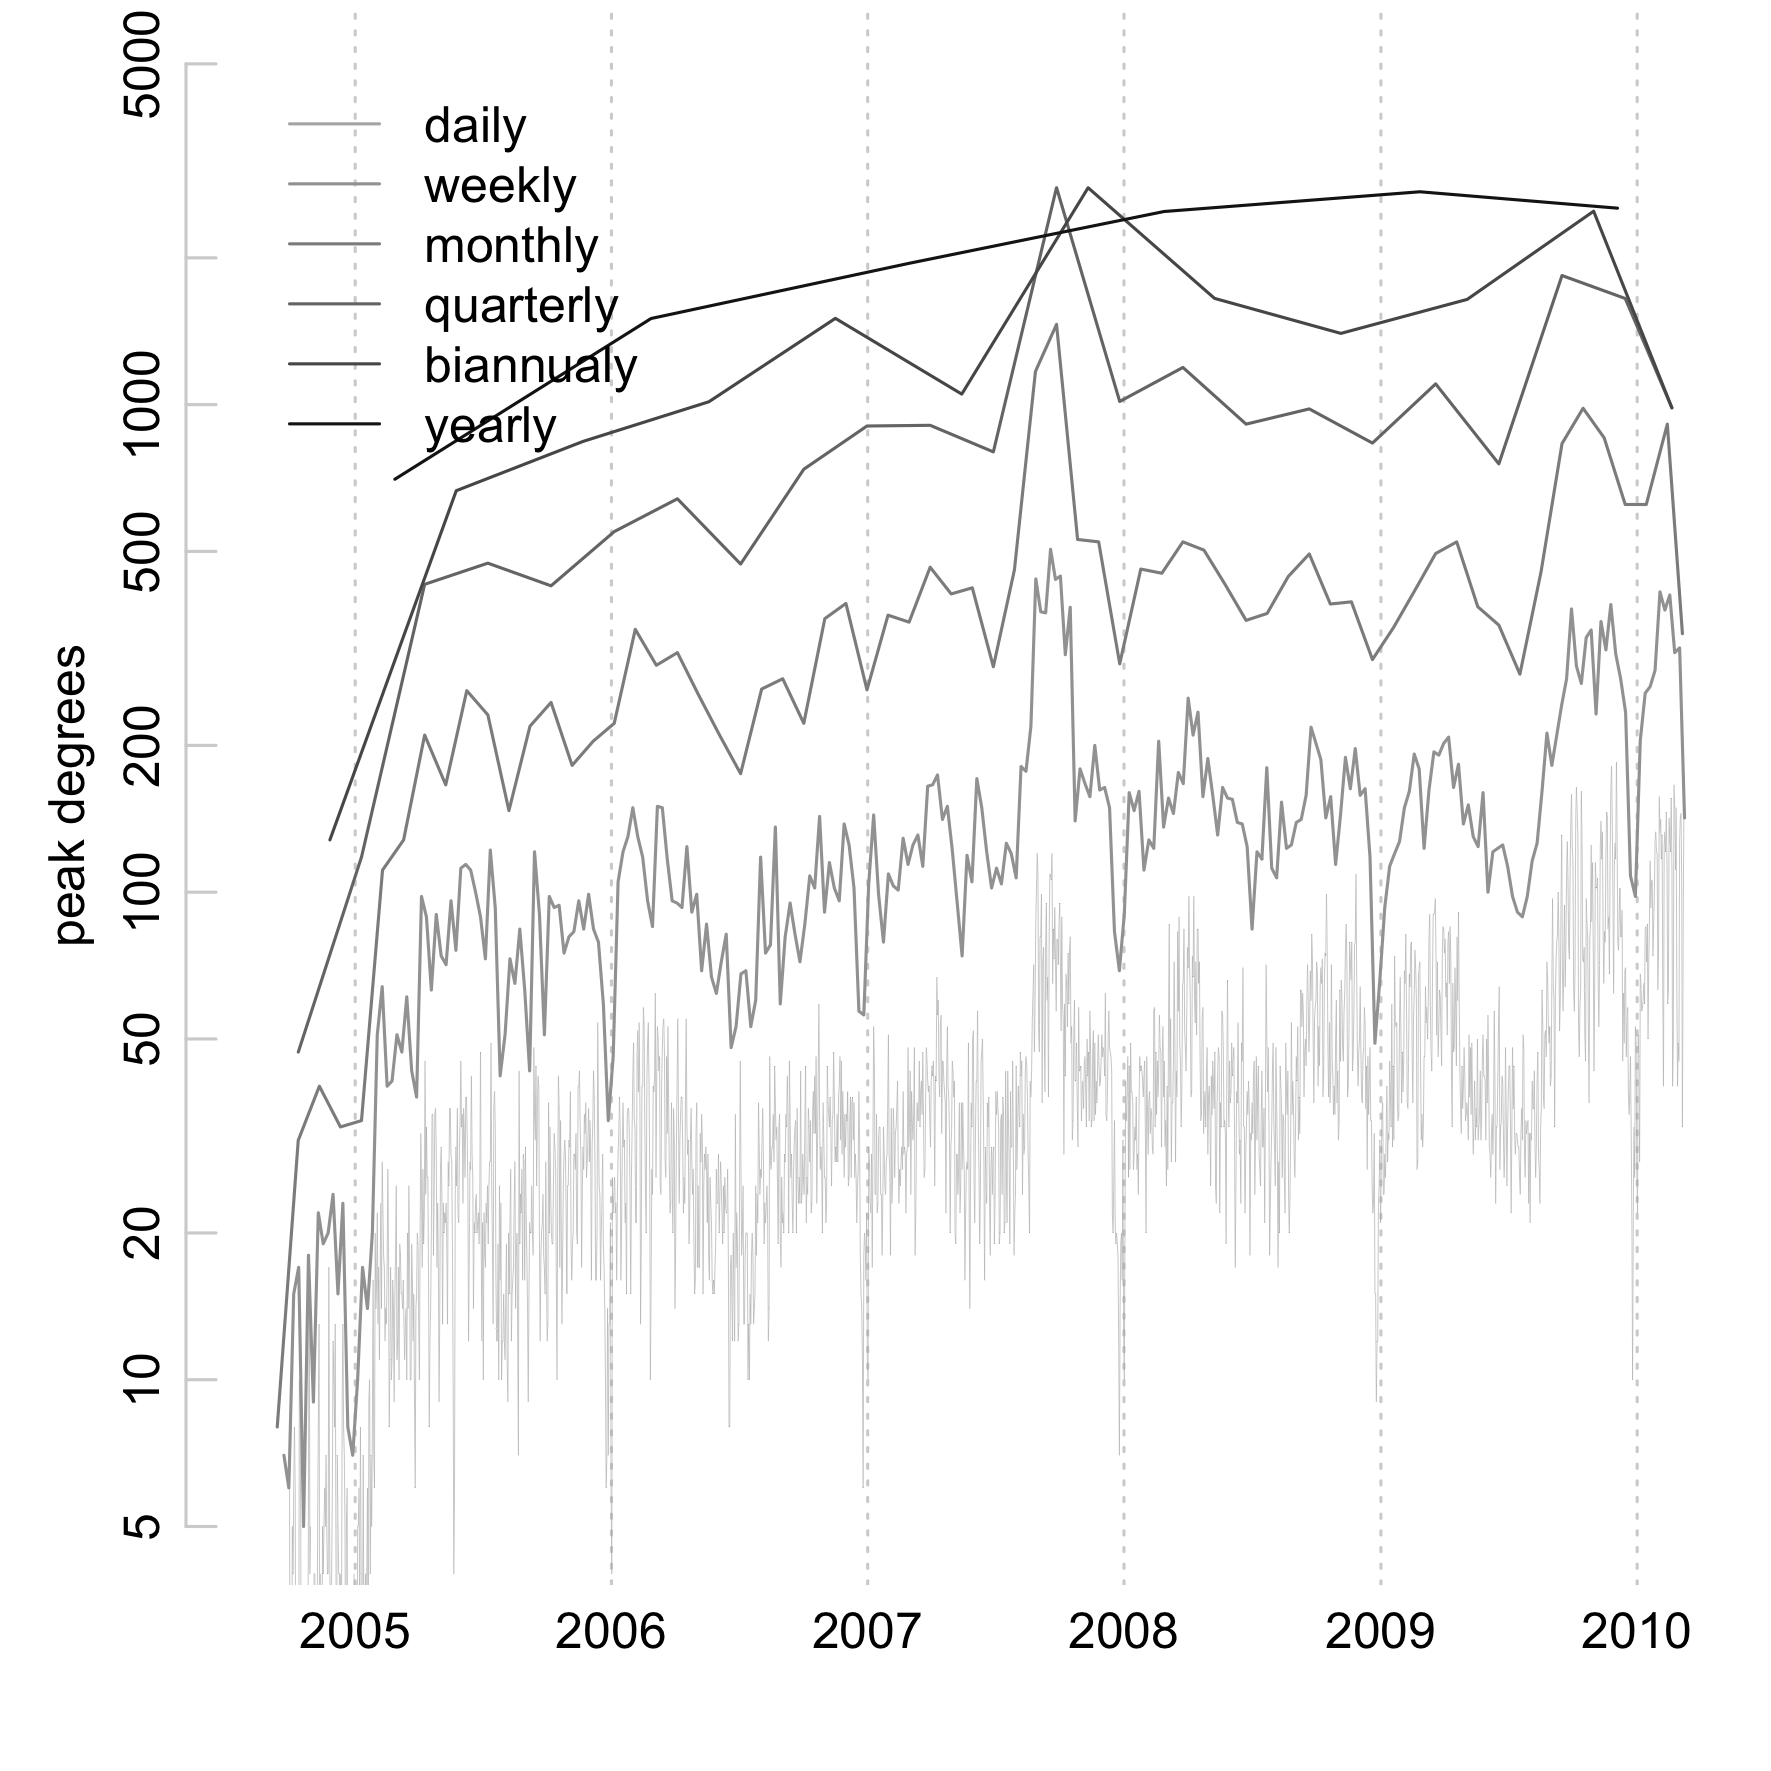
\includegraphics[width=1.0\linewidth]{maxEdges.png}
      \end{figure}   
    \end{oneCol}
    \end{columns}
    The WiFi access data have several notable trends.  First, the observed system usage, even after merging all duplicates, still increases by orders of magnitude, which is hardly reflected in the population change of any major metropolitan area during the same time.  The effect of the end boundary is also evident in the net users and locations.  Finally, the seasonal usage patterns are quite clear, even against the background trend. 
    \end{block}
    
    \begin{block}{Results}
    \begin{columns}
    \begin{oneCol}
      \setcounter{figure}{0}
      \begin{figure}
        \caption{Contacts Binned Daily}
        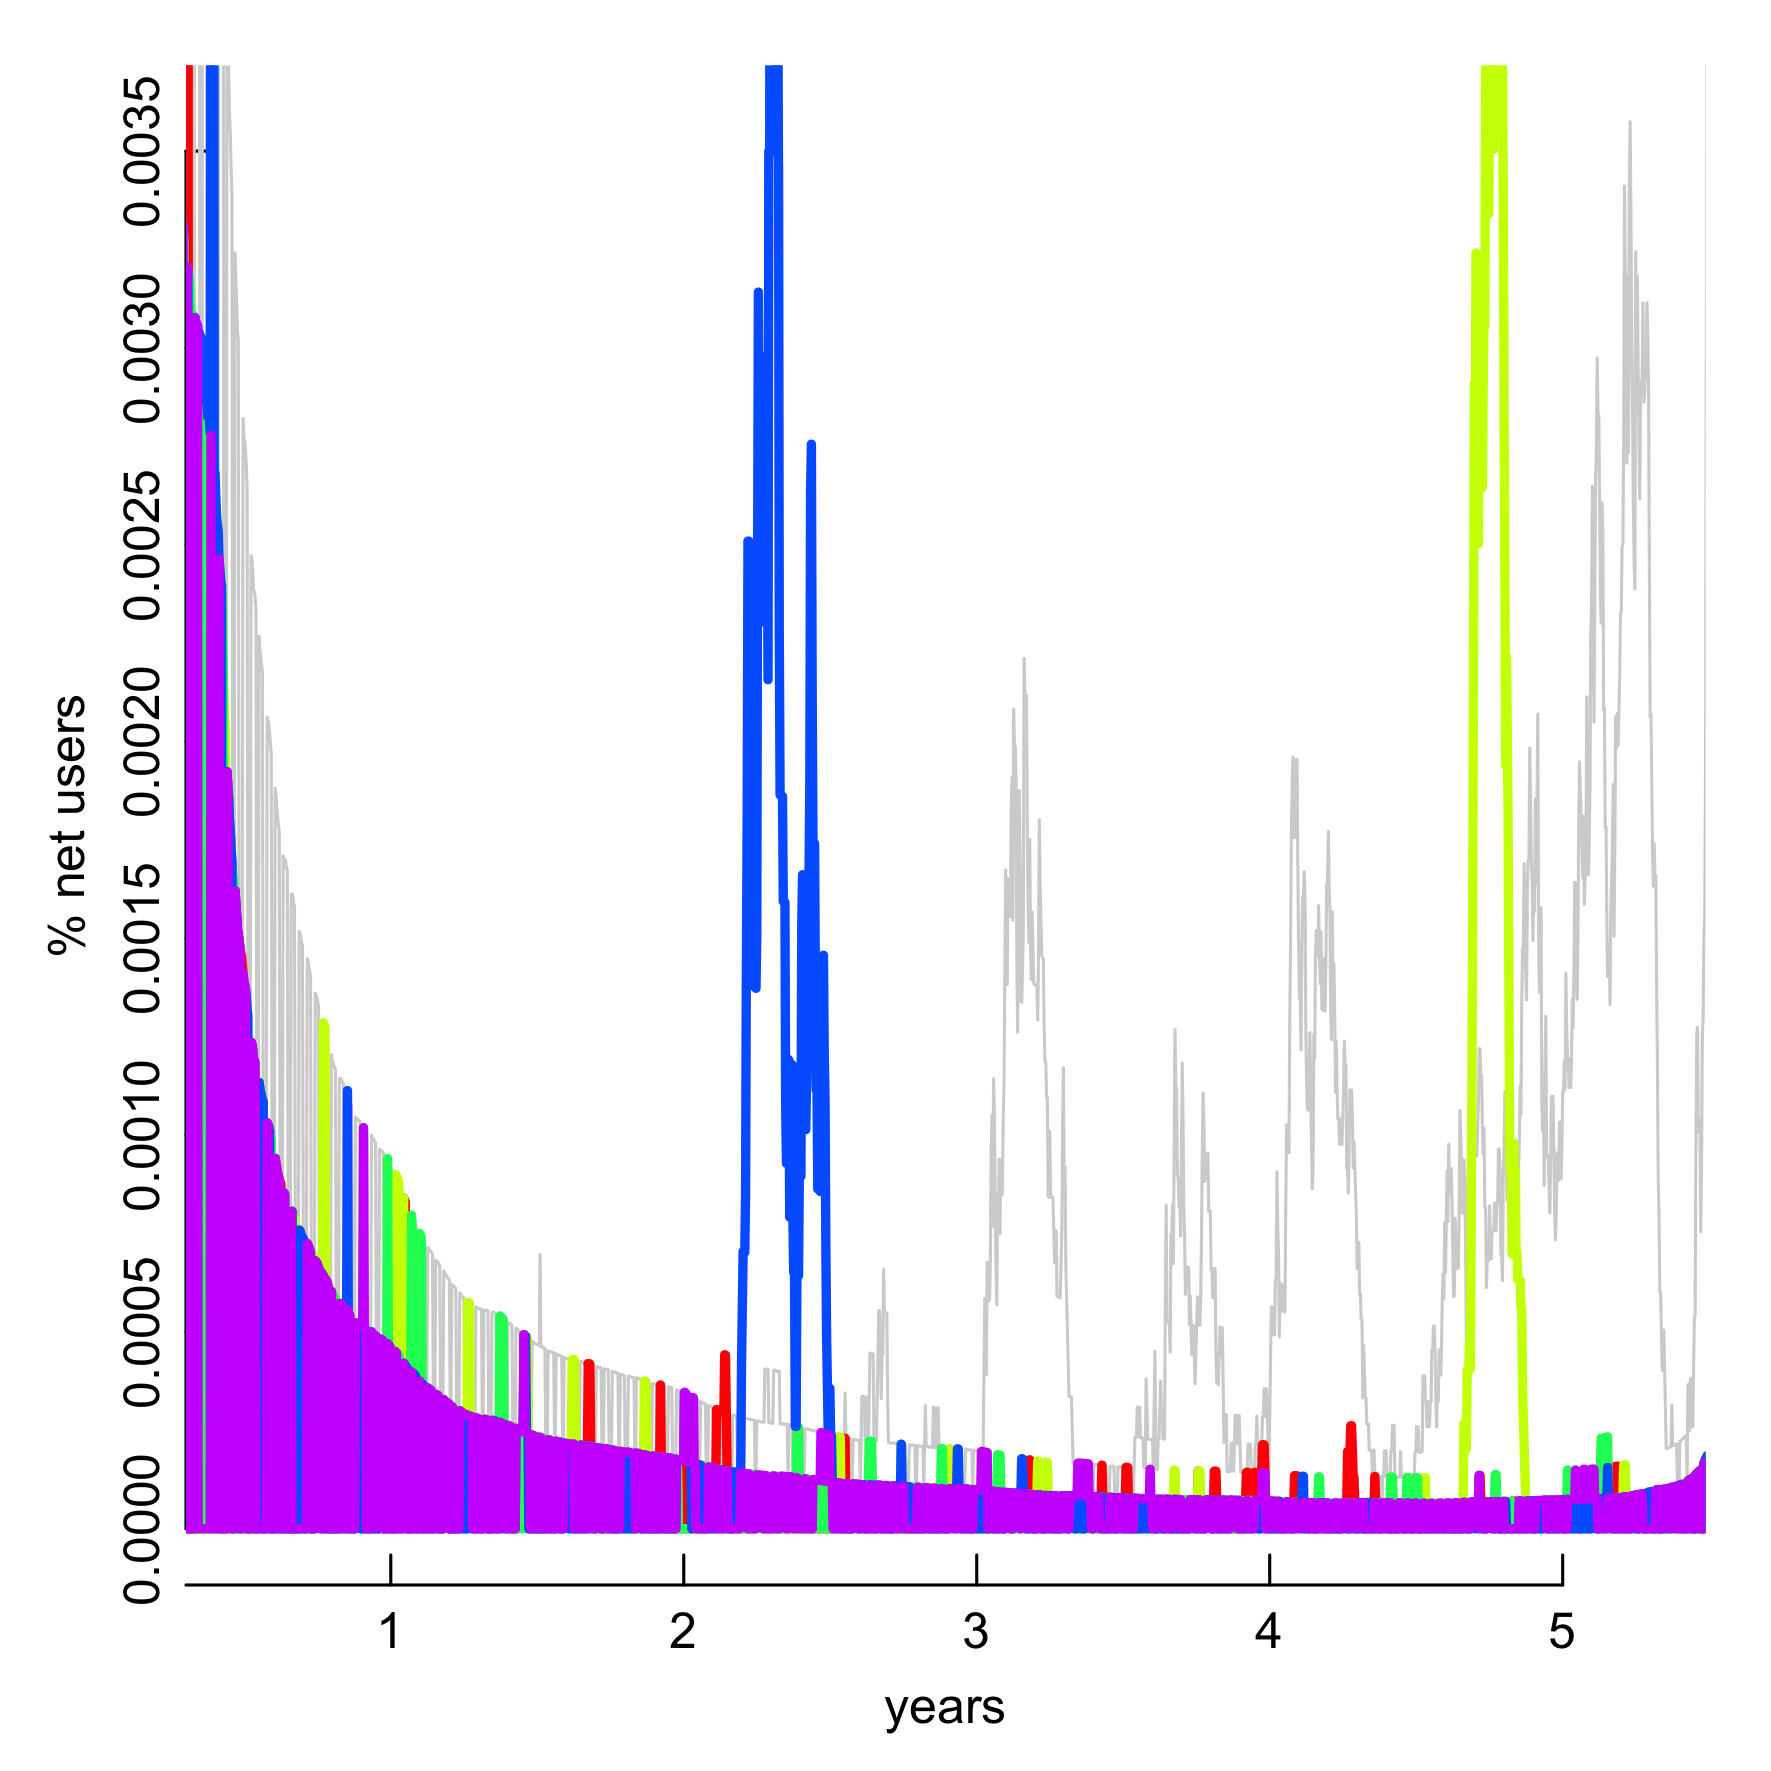
\includegraphics[width=1.0\linewidth]{out1.png}
      \end{figure}
      \setcounter{figure}{3}
      \begin{figure}
        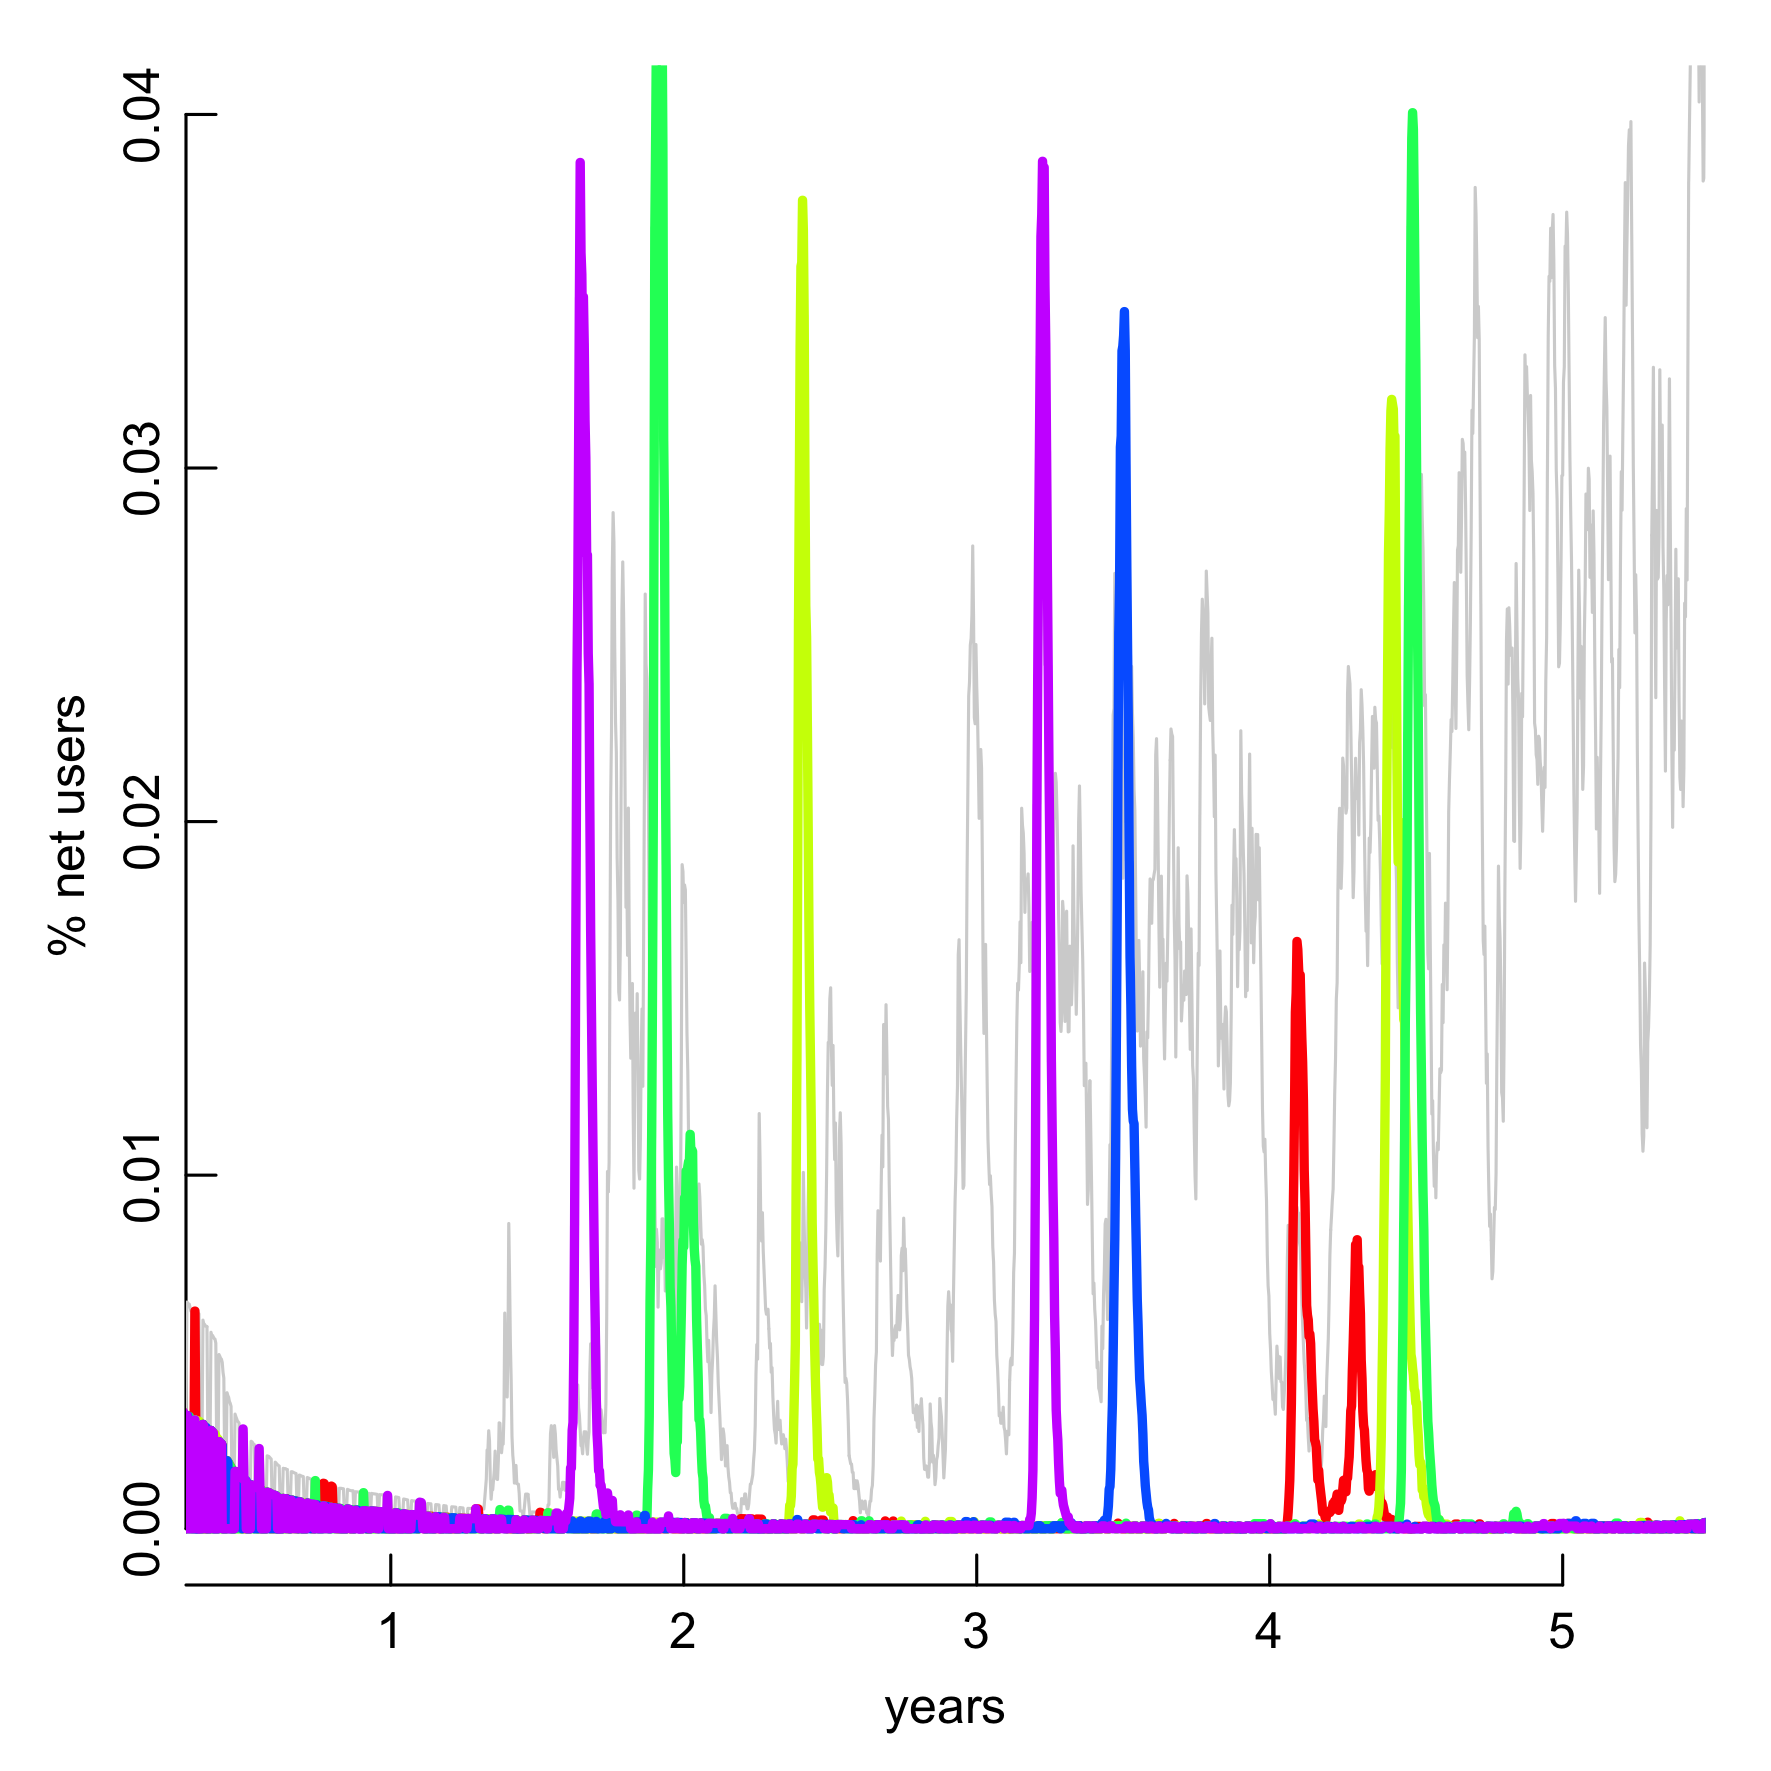
\includegraphics[width=1.0\linewidth]{out90.png}
        \caption{Contacts Binned Quarterly}
      \end{figure}  
    \end{oneCol}
    %\spacer{}
    \begin{oneCol}
      \setcounter{figure}{1}
      \begin{figure}
        \caption{Contacts Binned Weekly}
        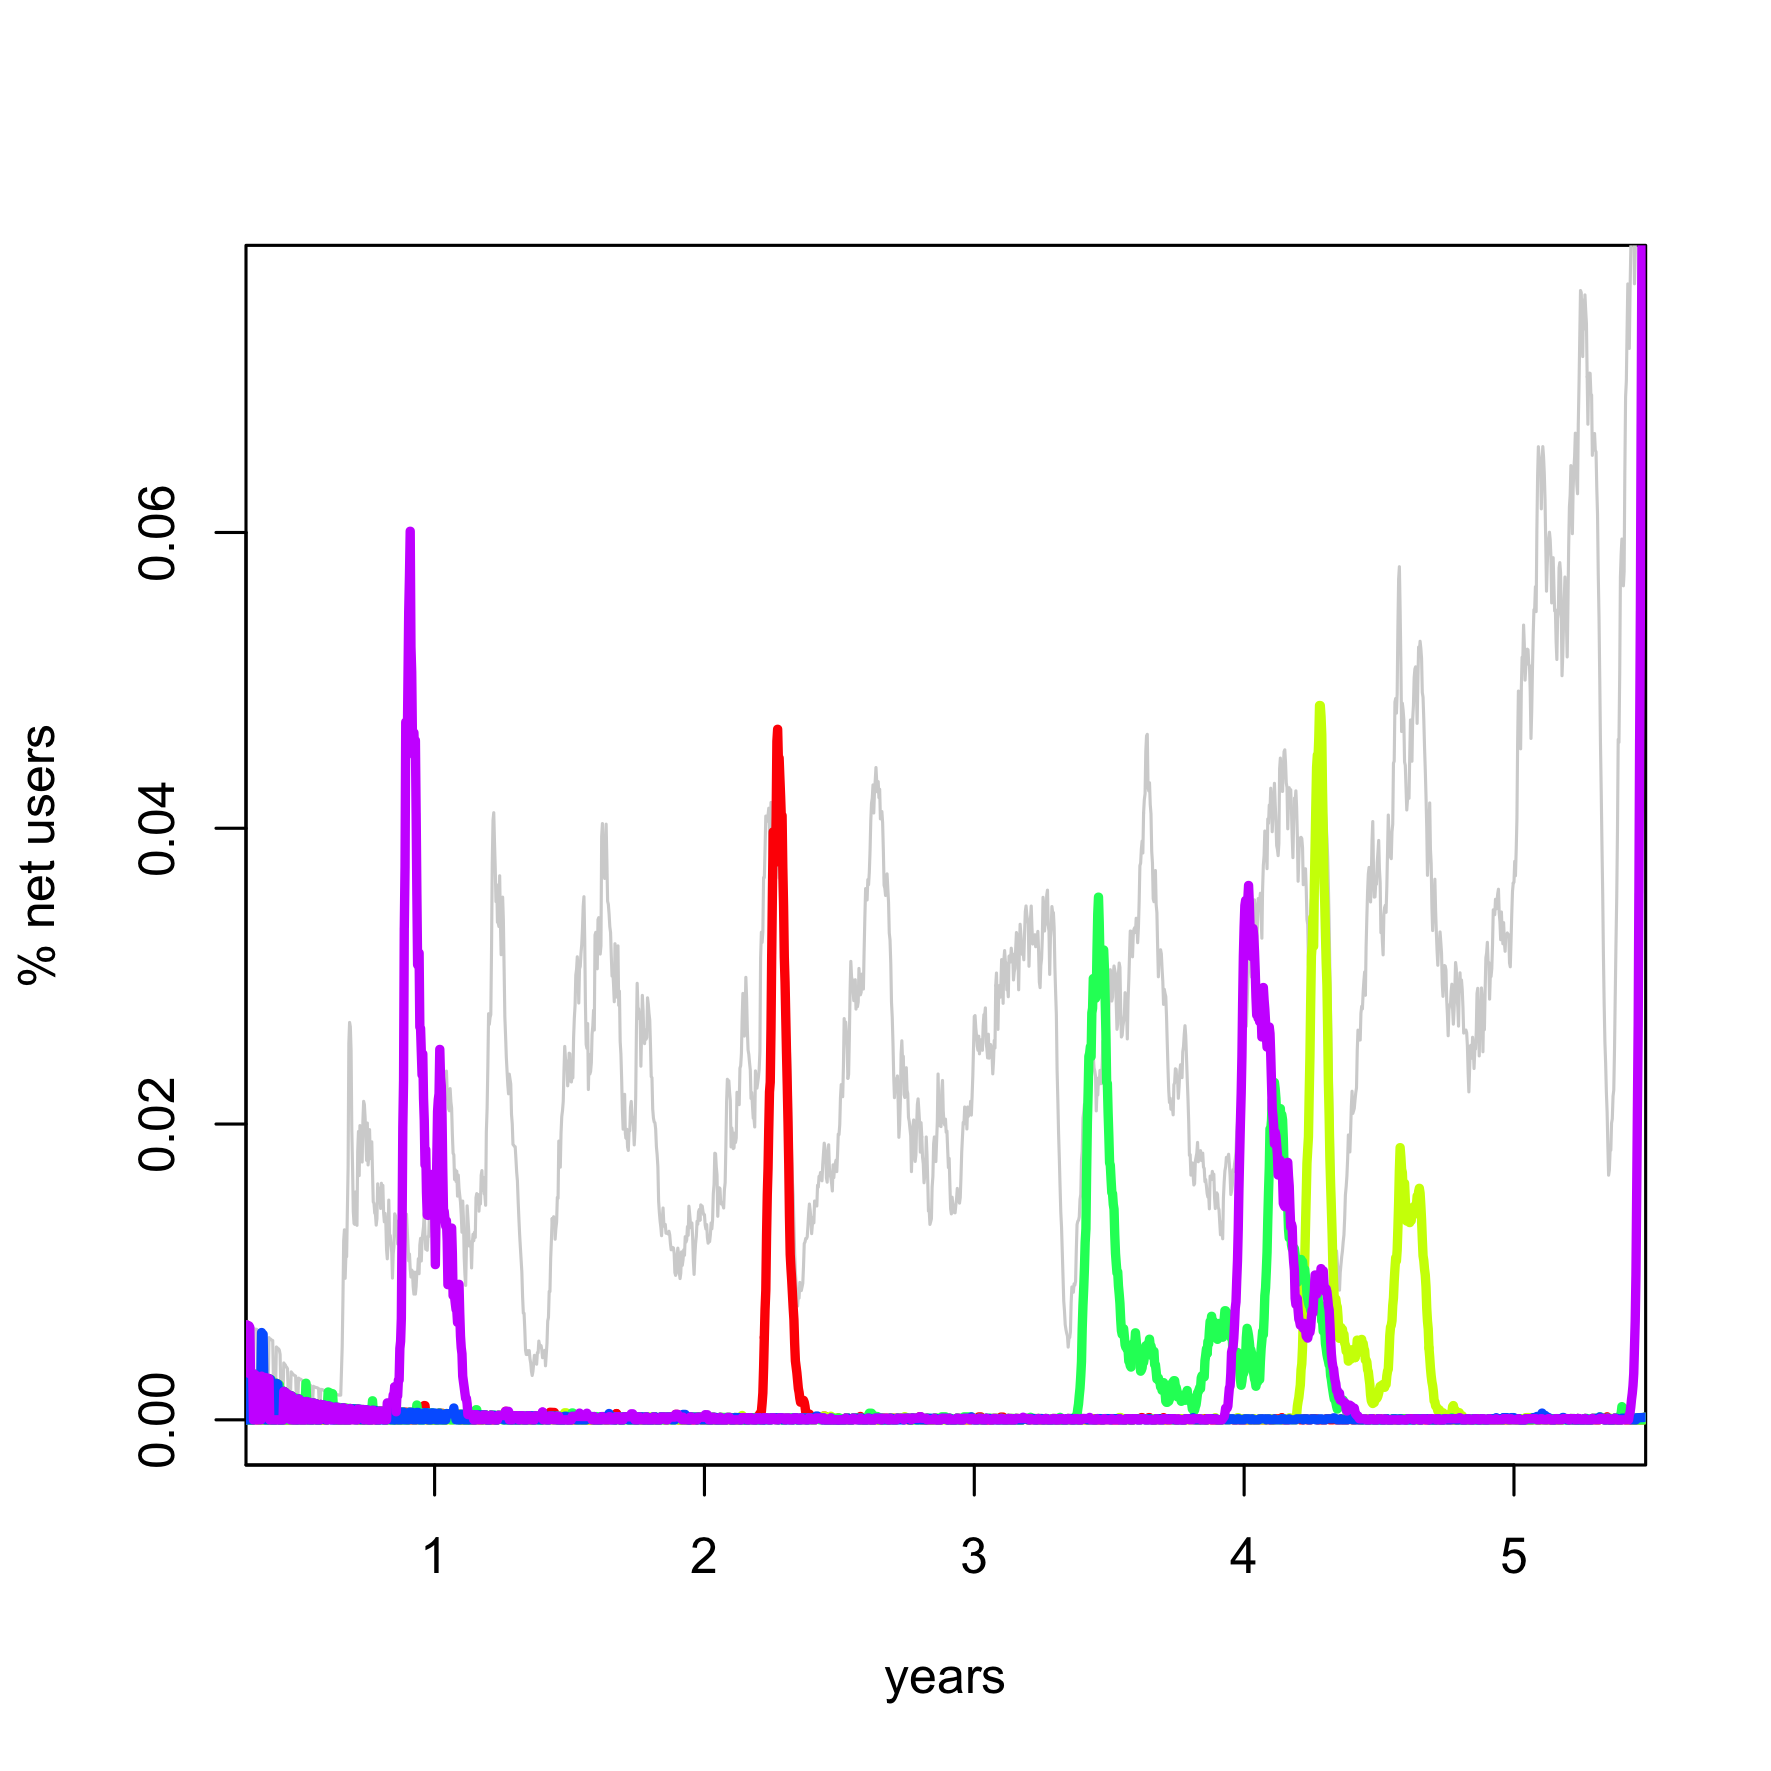
\includegraphics[width=1.0\linewidth]{out7.png}
      \end{figure}
      \setcounter{figure}{4}
      \begin{figure}
        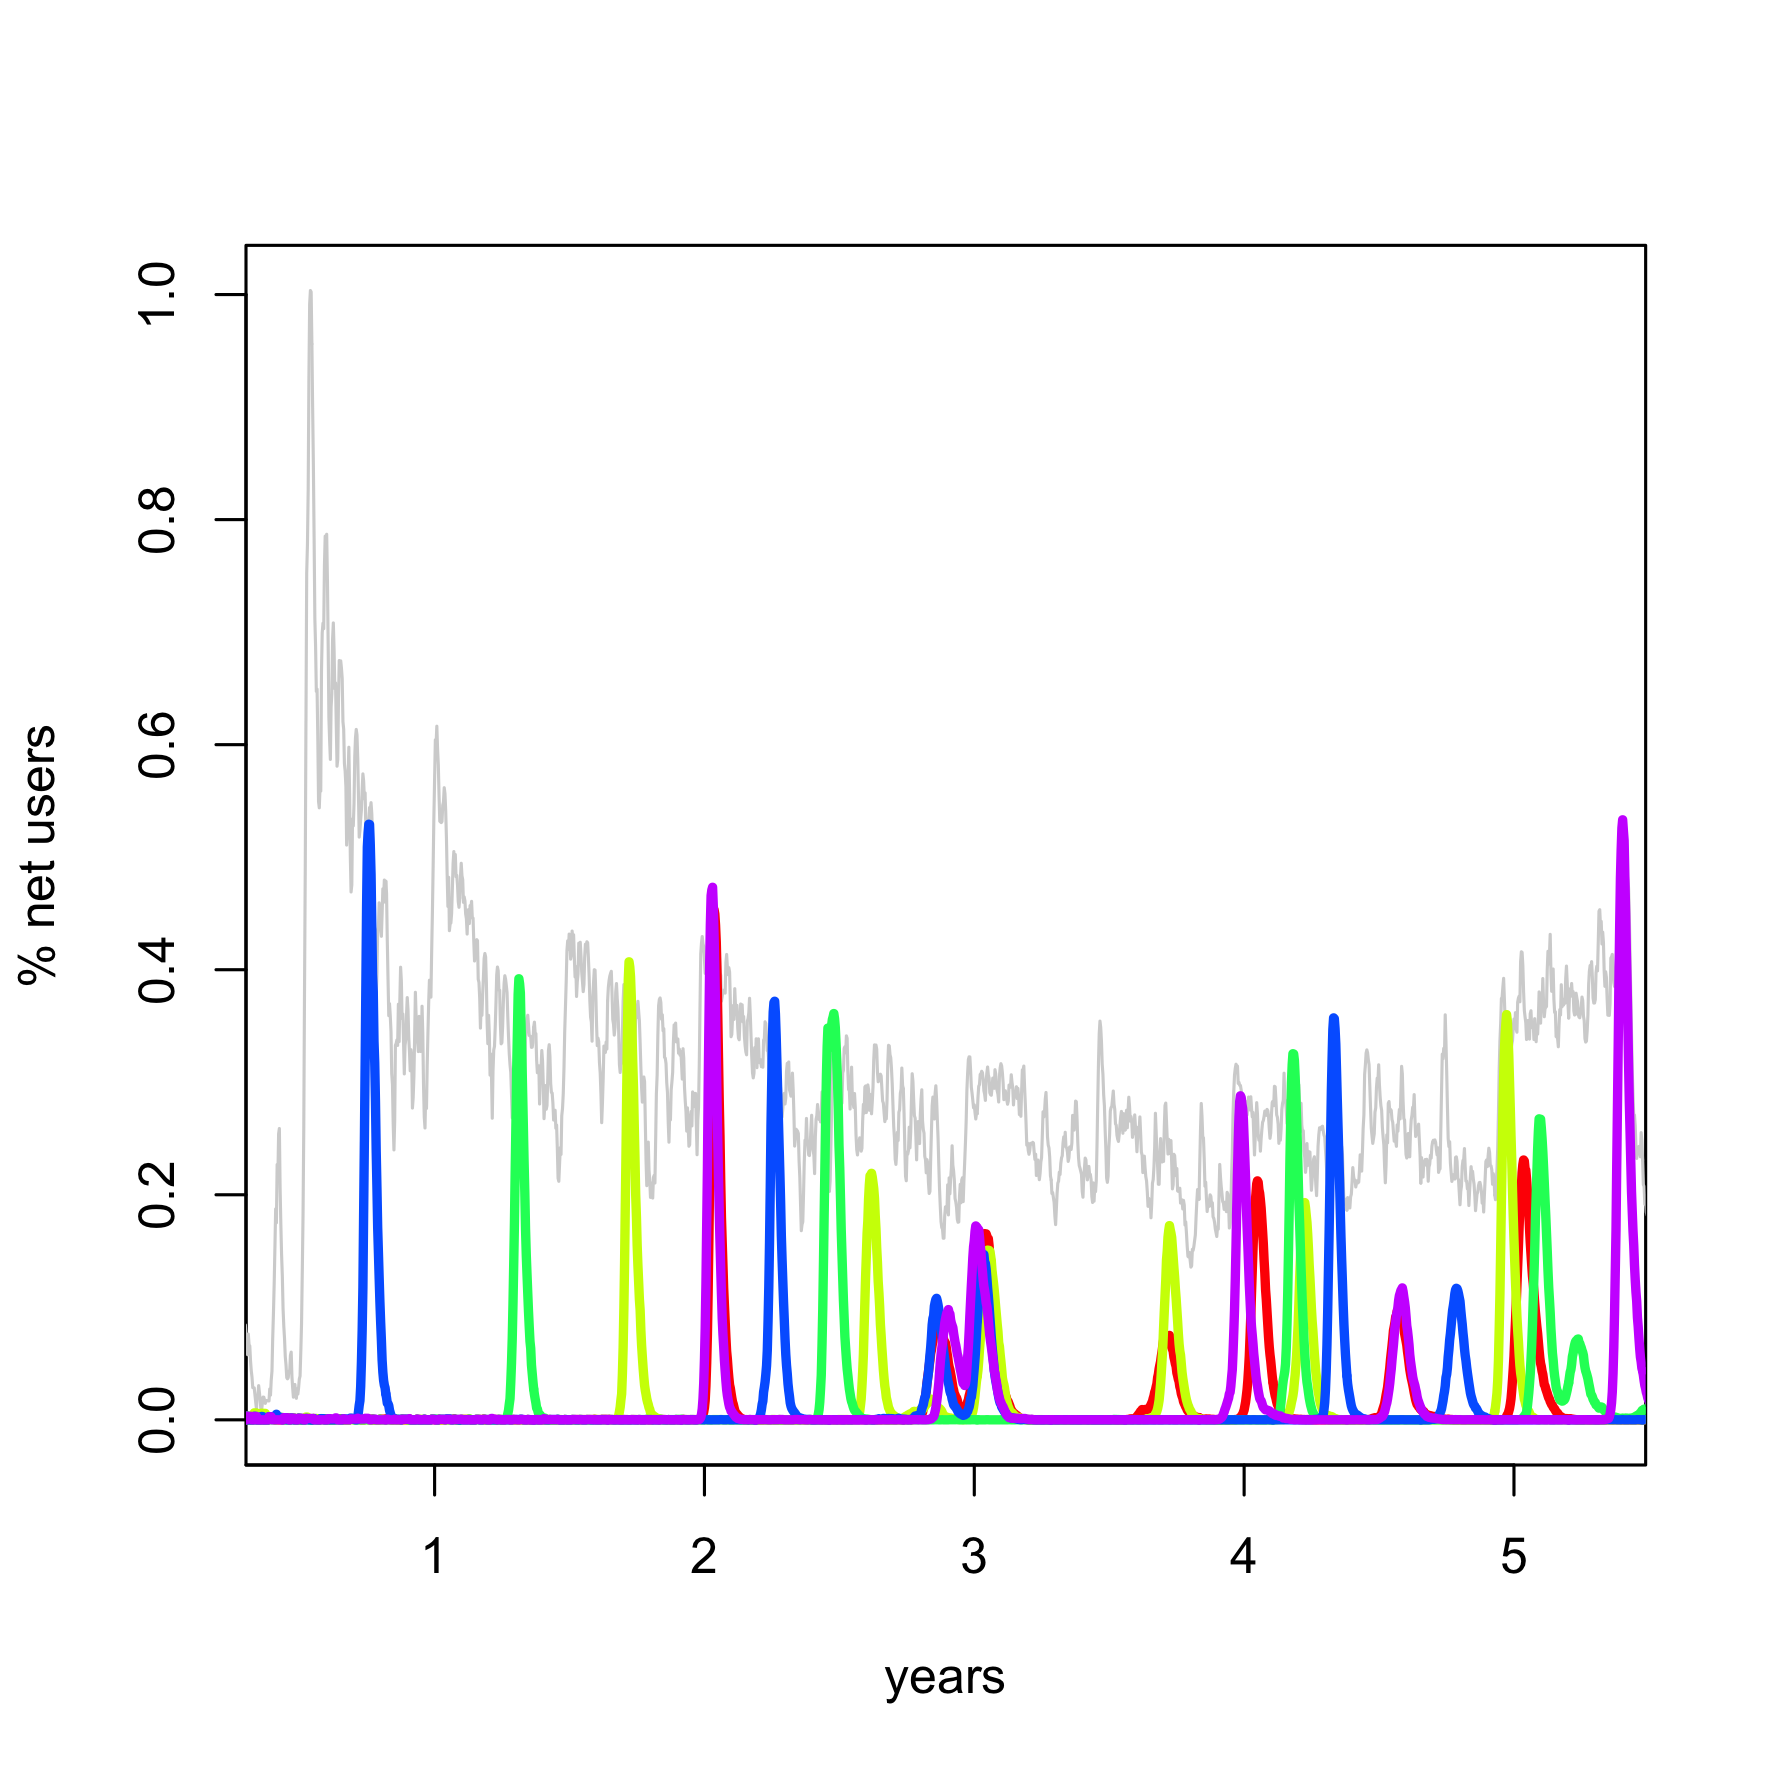
\includegraphics[width=1.0\linewidth]{out180.png}
        \caption{Contacts Binned Biannually}
      \end{figure}  
    \end{oneCol}
    %\spacer{}
    \begin{oneCol}
      \setcounter{figure}{2}
      \begin{figure}
        \caption{Contacts Binned Monthly}
        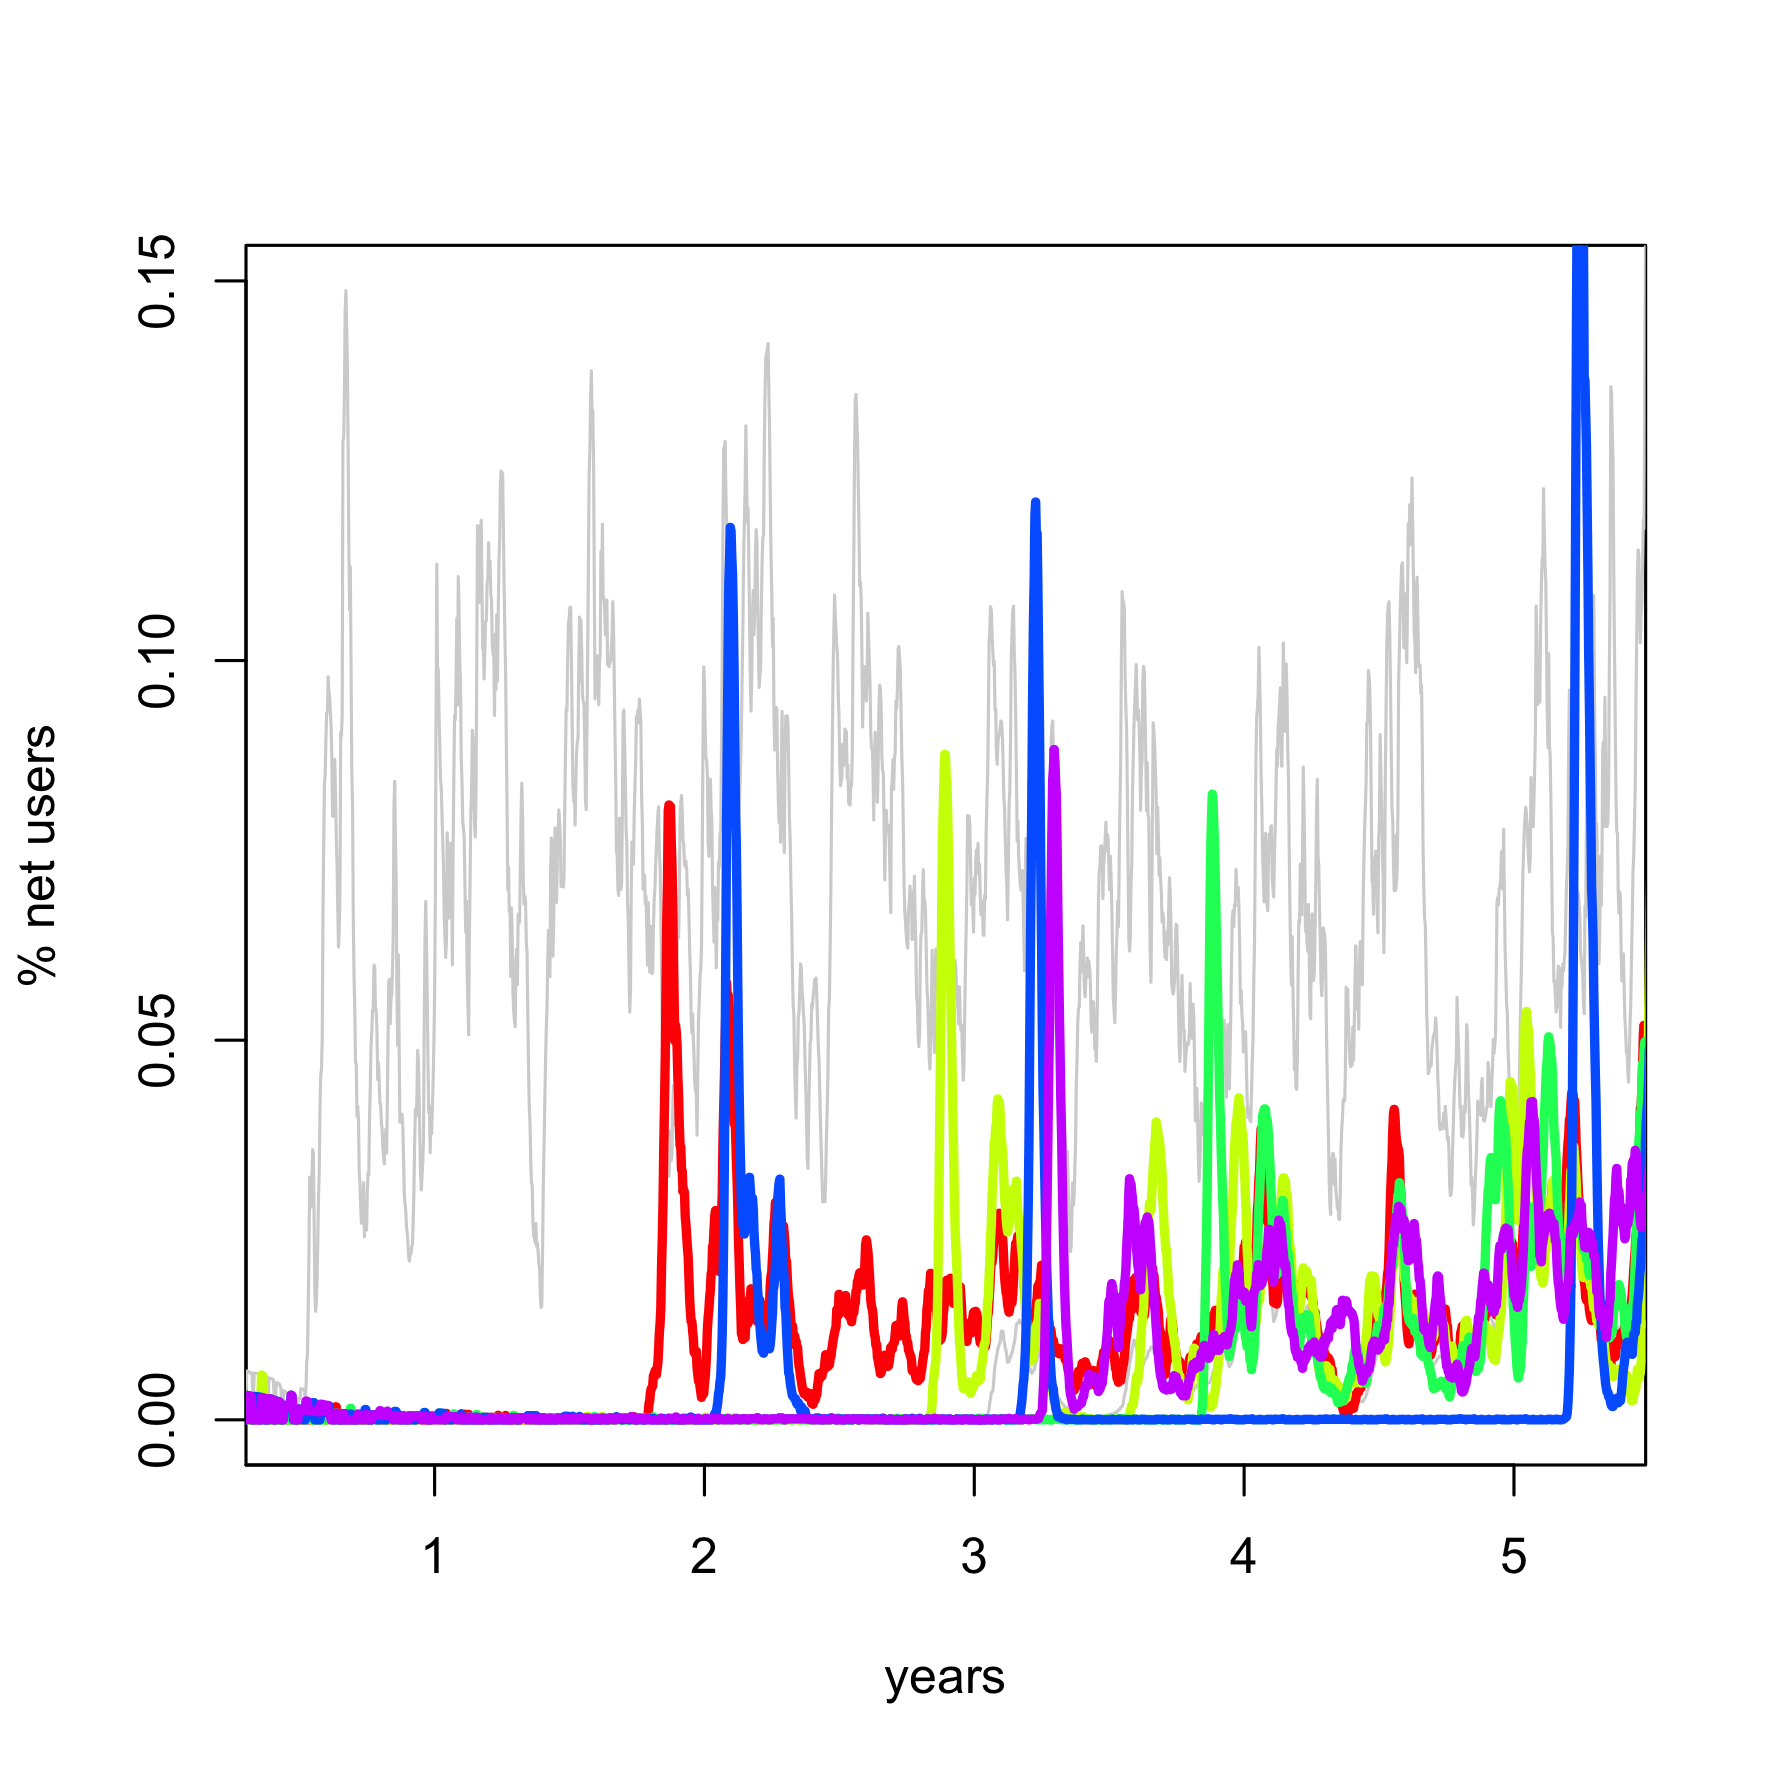
\includegraphics[width=1.0\linewidth]{out30.png}
      \end{figure}
      \setcounter{figure}{5}
      \begin{figure}
        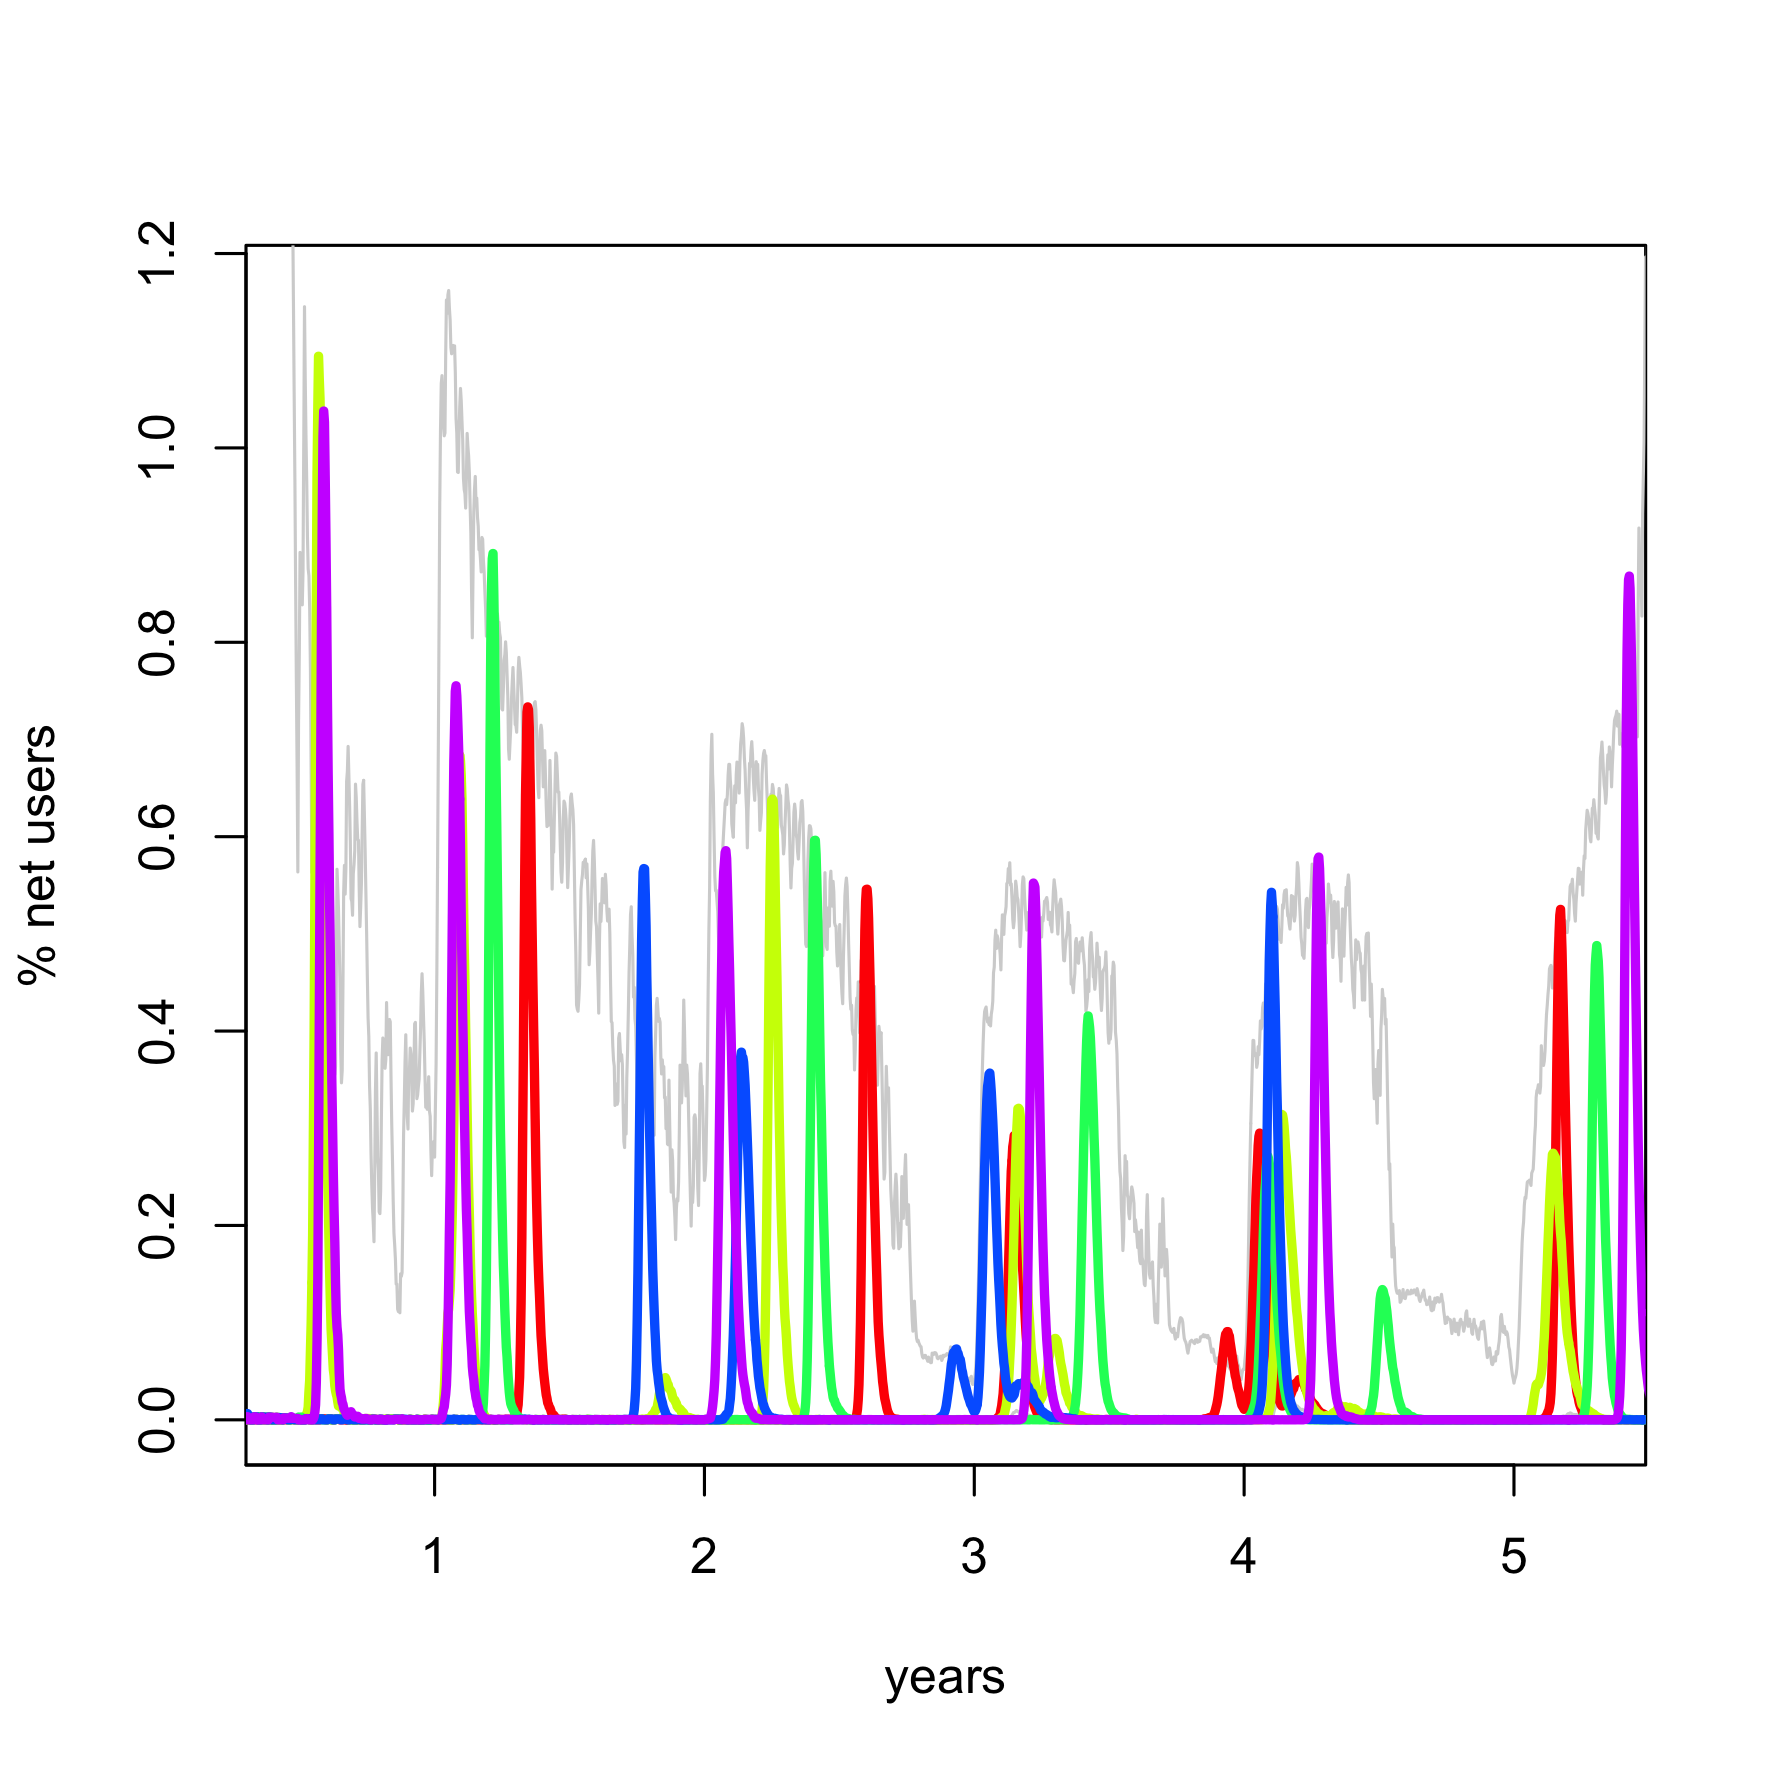
\includegraphics[width=1.0\linewidth]{out365.png}
        \caption{Contacts Binned Yearly}
      \end{figure}  
    \end{oneCol}
    \end{columns}
    \end{block}
    \begin{block}{Discussion}
    For the daily re-alignment of connections (Fig. 1), epidemics are rare, likely because the network is too sparsely connected at this aggregation level.  For the weekly re-alignment (Fig. 2), epidemics typically occur once per simulation, in waves that correspond to the seasonal dynamics in the raw data.  With the monthly re-alignment (Fig. 3), sustained transmission becomes possible, often with biannual peaks.  For the larger quarterly window (Fig. 4), epidemics are usually single-peaked. Large epidemics do not occur close together, perhaps because of the duration of herd immunity.  For the biannual bins (Fig. 5), epidemics are common, but do not occur more than once per 180-day bin. Apparent two-wave epidemics are likely artifacts of binning.  For the full year bins (Fig. 6), epidemics tend to be large and occur shortly after the beginning of the year, when edges have been updated. Updated edges may bring susceptible individuals into large components, marginalizing population-level immunity. Immunity duration prevents multiple epidemics per year.
    \end{block}
    \end{threeCol}
    \spacer{}
    \end{columns}
  \end{frame}
  \end{document}
